\chapter{Nuclear Physics}
\label{chapter:nuclear}

%\section[Nucleus]{Nucleus of the Atom}
%
%\begin{frame}{The Rutherford-Bohr Model}
%  Since Rutherford's and Bohr's atomic models, we know that the atom consists
%  of 
\begin{itemize}
\item A dense positively-charged nucleus
\item Almost all the mass is concentrated at the nucleus
\item Negatively-charged electrons ``orbiting'' the nucleus in predefined
  energy levels
\item Most of the atom is empty space

\end{itemize}
The nucleus
%---where most of the mass of the atom is concentrated---
are made up of \textbf{nucleons} which are:
\begin{itemize}
\item Positively charged \textbf{protons}, and 
\item Electrically neutral \textbf{neutrons}
\end{itemize}




%\section{Balancing Act}
The nucleus of an atom is held together by balancing two fundamental forces:
\begin{center}
  \pic{.3}{nuclearPhysics/graphics/Nuclear_force}
\end{center}
\textbf{Electromagnetic force}
\begin{itemize}
\item the repulsive force between protons
\item Force drop off as $1/r^2$ (inverse square law)
  but have infinite range
\end{itemize}

\textbf{Strong nuclear force}
\begin{itemize}
\item Short-distance force between nucleons
\item Attractive at about $\SI1{\femto\metre}$ (\SI{e-15}\metre)
\item Repulsive at distances below \SI{.7}{\femto\metre}
\item Insignificant at distances beyond \SI{2.5}{\femto\metre}
  %\item 137 times stronger than electromagnetic force inside the nucleus
\end{itemize}
  




\section{Atomic Properties}
  The nucleus of an atom is identified by two integers:
  \begin{center}
    \begin{tikzpicture}[auto,node distance=140, thick]
      \node (he) {\fontsize{60}{70}\isotope[4][2]{He}};
      \node[font=\large] (name) [right of=he] {element symbol};
      \draw[axes] (name)--(he);
      \node[left,font=\large] (A) at (-2,.5) {mass number};
      \node[left,font=\large] (Z) at (-2,-.5) {atomic number};
      \draw[axes] (A)--(-1.3,.5);
      \draw[axes] (Z)--(-1.3,-.5);
    \end{tikzpicture}
  \end{center}
  \begin{itemize}
  \item\textbf{Atomic number} ($Z$): the number of protons
    \begin{itemize}
    \item Determines what element it is, and
    \item Determines the number of electrons an atom would have, and therefore
    \item its chemical properties
    \end{itemize}
  \item\textbf{Mass number} ($A$): number of nucleons
  \item The number of neutrons ($N$) is therefore $N=A-Z$
  \end{itemize}




\section{Isotopes}
Carbon has three common \textbf{isotopes}, all with the same atomic numbers,
but different number of neutrons (called ``carbon-12'', ``carbon-13'' and
``carbon-14'' respectively):\footnote{The atomic number is often omitted
for common elements. }
\begin{displaymath}
  \isotope[12]{C}\quad\isotope[13]{C}\quad\isotope[14]{C}
\end{displaymath}

Hydrogen has three naturally-occurring isotopes: protium, deuterium and tritium.
Protium (hydrogen-1) and deuterium (hydrogen-2) are
stable\footnote{i.e.\ they do not undergo radioactive decay}, but tritium
(hydrogen-3) has a half-life of 13.2 years
\begin{displaymath}
  \isotope[1]{H}\quad\isotope[2]{H}\quad\isotope[3]{H}
\end{displaymath}
On average, there are 2.6 stable isotopes for each element.



\section{Mass of the Nucleus}
The \textbf{unified atomic mass unit} (\si{u})\footnote{Same as the
``atomic mass unit'' (\si{amu}) used in chemistry classes. The atomic mass
value in the periodic table is a weighted average across all isotopes.} is
defined as $1/12$ of the rest mass of a \isotope[12]{C} atom in its nuclear
ground state:
\begin{equation}
  \SI1{u}=\frac1{12}m(\isotope[12]{C})\approx\SI{1.66054e-27}{\kilo\gram}
\end{equation}
The rest mass of the elementary particles can be expressed in this unit:
\begin{center}
  \begin{tabular}{l|l|l}
    \rowcolor{pink}
    \textbf{Particle} & \textbf{Mass} (\si{u}) & \textbf{Mass} (\si{kg})\\
    \hline
    Proton   & \num{1.007276} & \num{1.672614e-27} \\
    Neutron  & \num{1.008665} & \num{1.674920e-27} \\\hline
    Electron & \num{0.000549} & \num{9.10956e-31}
  \end{tabular}
\end{center}

\begin{itemize}
\item The unified atomic mass unit is related to Avogadro's constant ($N_A$)
  in Chemistry. $N_A$ is historically defined as a number of atoms in
  \SI{12}{\gram} of \isotope[12]C, called \SI1\mol.

  \begin{equation}
    N_A=\frac1{\num{1.66054e-24}}=\num{6.02214e23}
  \end{equation}

\item When you sum the masses of 6 protons, 6 neutrons and 6 electrons using
  the values given to you on the previous slide, you will get:
  \begin{equation}
    6m_P+6m_N+6m_e=\SI{12.09894}{u}
  \end{equation}
  This is \emph{more} than \SI{12}{u}!
\end{itemize}
%
%
%
%
%\section[Mass Defect]{Mass Defect \& Nuclear Binding Energy}

\section{Mass-Energy Equivalence}
One of the discoveries in special relativity\footnote{Einstein, A., ``Does
the Inertia of a Body Depend Upon Its Energy Content?'', \emph{Annelen der
Physik}, 18(13):639-641, 21 November, 1905.} is the fundamental equivalence
of mass and energy. While it is derived based on
\emph{relativistic kinematics}, it also applies to \emph{quantum mechanics},
from which nuclear physics is based on.
\begin{equation*}
  E=mc^2
\end{equation*}
\begin{center}
  \begin{tabular}{l|c|c}
    \rowcolor{pink}
    \textbf{Quantity} & \textbf{Symbol} & \textbf{SI Unit} \\ \hline
    Energy                  & $E$ & \si\joule \\
    Rest mass of a particle & $m$ & \si{\kilo\gram}\\
    Speed of light          & $c$ & \si{\metre\per\second}
  \end{tabular}
\end{center}
The speed of light is a universal constant: $c=\SI{2.998e8}{\metre\per\second}$.
%  \vspace{.3in}
%
%
%
%
%
%\section{Mass-Energy Equivalence}
A change in energy $\Delta E$ is \emph{always} accompanied by a change in
mass $\Delta m$, and vice versa:
\begin{equation}
  E=mc^2\quad\to\quad\Delta E=\Delta mc^2
\end{equation}
\begin{itemize}
\item The concept is difficult to visualize in everyday life
\item For example: a car travelling at \SI{30}{\metre\per\second}
  (\SI{108}{\kilo\metre\per\hour}) is more massive than when it is
  stationary\footnote{As a simple example, calculate the additional mass a
  \SI{2000}{\kilo\gram} car would have while travelling at
  \SI{30}{\metre\per\second}.}, but $\Delta m$ is too small to be measured
\item But the difference is more significant when
  \begin{itemize}
  \item speeds approaches the speed of light ($v>0.3c$), or when
  \item the masses are small (e.g.\ electrons, protons, neutrons)
  \end{itemize}
\end{itemize}
%
%
%
%
\section{Mass Defect}

The sum of the masses of the individual nucleons are \emph{always} higher
than the mass of the nucleus itself. For example, the mass of the alpha
particle (helium-4 nucleus) is lower than 2 protons plus 2 neutrons:
\begin{center}
  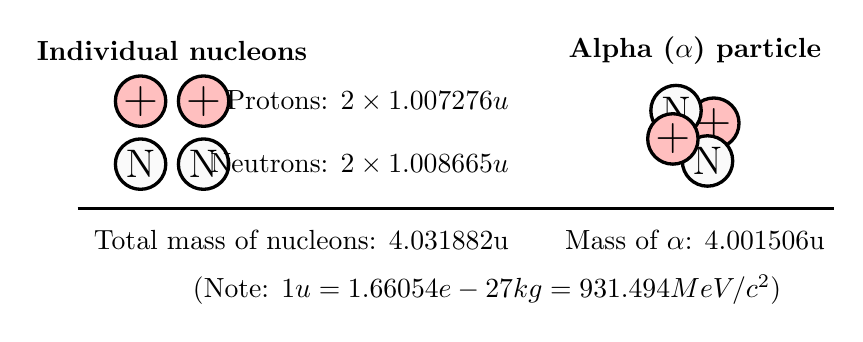
\begin{tikzpicture}[scale=.8]
    \node at (.5,.8) {\textbf{Individual nucleons}};
    \draw[very thick,fill=pink] circle (.4) node{\LARGE$+$};
    \draw[very thick,fill=pink] (1,0) circle (.4) node{\LARGE$+$};
    \draw[very thick,fill=black!2] (0,-1) circle (.4) node{\Large N};
    \draw[very thick,fill=black!2] (1,-1) circle (.4) node{\Large N};
  
    \draw[very thick] (-1,-1.7)--+(12,0);
    
    \node[left] at (6,0) {Protons: $2\times\SI{1.007276}u$};
    \node[left] at (6,-1) {Neutrons: $2\times\SI{1.008665}u$};
    \node[left] at (6,-2.2) {Total mass of nucleons: \SI{4.031882}u};

    \draw[very thick,fill=pink] (9.1,-.35) circle (.4) node{\LARGE$+$};
    \draw[very thick,fill=black!2] (8.5,-.15) circle (.4) node{\Large N};
    \draw[very thick,fill=black!2] (9,-.95) circle (.4) node{\Large N};
    \draw[very thick,fill=pink] (8.45,-.6) circle (.4) node{\LARGE$+$};

    \node at (8.8,.8) {\textbf{Alpha ($\alpha$) particle}};
    \node at (8.8,-2.2) {Mass of $\alpha$: \SI{4.001506}u};

    \node at (5.5,-3) {
      (Note: $\SI1u=\SI{1.66054e-27}{kg}=\SI{931.494}{MeV/c^2}$)
    };
  \end{tikzpicture}
\end{center}

This difference in mass is called the \textbf{mass defect} ($\Delta m$), which
can be calculated with a simple equation:
\begin{equation}
  \Delta m=\left[Zm_P+(A-Z)m_N\right]-m_A
\end{equation}
\begin{center}
  \begin{tabular}{l|c|c}
    \rowcolor{pink}
    \textbf{Quantity} & \textbf{Symbol} & \textbf{SI Unit} \\ \hline
    Mass defect       & $\Delta m$ & \si{\kilo\gram}\\
    Atomic number and mass numbers & $Z$, $A$ & \\
    Rest mass of a proton and neutron & $m_P$, $m_N$ & \si{\kilo\gram}\\
    Rest mass of the nucleus & $m_A$ & \si{\kilo\gram}\\
  \end{tabular}
\end{center}
Mass defect exists in all nuclei because the nucleus of an atom is always
\emph{in a lower energy state} than the individual nucleons alone

Similar examples:
\begin{itemize}
\item The total energy of a planet orbiting the Sun is lower than the planet
  and the Sun individually
\item An electron orbiting the nucleus is at a lower energy state also
\end{itemize}



\section{Nuclear Binding Energy}

The amount of energy that is equivalent to the mass defect is called the
\textbf{nuclear binding energy} $E_b$, defined as:
\begin{equation}
  \boxed{E_b=(\Delta m)c^2}
\end{equation}
\begin{center}
  \begin{tabular}{l|c|c}
    \rowcolor{pink}
    \textbf{Quantity}      & \textbf{Symbol} & \textbf{SI Unit} \\ \hline
    Nuclear binding energy & $E_b$      & \si\joule \\
    Mass defect            & $\Delta m$ & \si{\kilo\gram}\\
    Speed of light         & $c$        & \si{\metre\per\second}
  \end{tabular}
\end{center}
\begin{itemize}
\item The energy (or external work) required to break up the nucleus
  %into its individual nucleons
\item Usually expressed in \emph{electron volts} (\si\electronvolt) where
  $\SI1\electronvolt=\SI{1.602e-19}\joule$ %, rather than in joules
\end{itemize}

%\section{Nuclear Binding Energy}
The nuclear binding energy is the amount of external work required to
separate the nucleons in the nucleus
\begin{center}
  \pic{.5}{nuclearPhysics/graphics/CNX_UPhysics_43_02_BindEnergy}
  
  \vspace{.3in}
  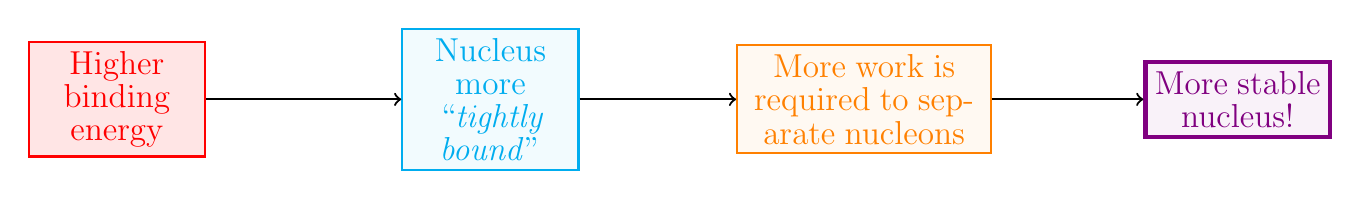
\begin{tikzpicture}[auto,node distance=135,thick]
    \node[
      text width=57,
      align=center,
      fill=red!10,
      draw=red] (a) {
      \large\color{red}{Higher binding energy}};
    \node[
      text width=57,
      align=center,
      fill=cyan!5,
      draw=cyan] (b) [right of=a]{
      \large\color{cyan}{Nucleus more ``\emph{tightly bound}''}};
    
    \node[
      text width=85,
      align=center,
      fill=orange!5,draw=orange] (c) [right of=b]{
      \large\color{orange}{More work is required to separate nucleons}};
    
    \node[
      line width=1.5,
      text width=60,
      align=center,
      fill=violet!5,draw=violet] (d) [right of=c]{
      \large\color{violet}{More stable nucleus!}};
    
    \draw[->] (a)--(b);
    \draw[->] (b)--(c);
    \draw[->] (c)--(d);
  \end{tikzpicture}
\end{center}
The higher the binding energy, the more \emph{tightly bound} a nucleus is,
therefore more work is required to separate the nucleons




%\section{Nuclear Binding Energy \& Stability of the Nucleus}
The nuclear binding energy is highest for \isotope[56]{Fe}
($E_b=\SI{492.275}{\mega\electronvolt}$, or \SI{8.7906}{\mega\electronvolt}
per nucleon)

%\pic1{nuclearPhysics/graphics/CNX_UPhysics_43_02_BindingEng}

It means that the nucleus
\begin{itemize}
\item requires the \emph{most} energy to separate the nucleons
\item \emph{most} tightly bound
\item \emph{most} stable
\end{itemize}
To achieve greater stability in the nucleus
\begin{itemize}
\item Heavier atoms can split into lighter nuclei, while
\item Lighter atoms can combine into heavier nuclei
\end{itemize}
  




\begin{example}
  Given that the mass of a lithium-7 atom is $m=\SI{7.01600}u$, determine its
  mass defect and binding energy.
\end{example}

\section{Radioactivity}
%
%%\section{Radioactive Decay}
%  \begin{itemize}
%  \item Heavier elements: protons are further apart, and
%    the strong nuclear force is weakened by their distance
%  \item The nucleus can spontaneously disintegrate and releases energy
%  \end{itemize}
%



%\section{Radioactive Decay}
\textbf{Radioactivity} (or \textbf{radioactive decay}) is the spontaneously
disintegration of a nucleus. There are \emph{three} types of radioactive
decay:
\begin{itemize}
\item\textbf{Alpha decay}, or $\alpha$-decay
\item\textbf{Beta decay}, or $\beta$-decay
\item\textbf{Gamma decay}, or $\gamma$-decay
\end{itemize}



\subsection{Alpha Decay}

In $\alpha$-decay, an \textbf{alpha particle} %(helium-4 nucleus, with 2
%protons and 2 neutrons),
is spontaneously emitted from the nucleus. Example:
plutonium-240 nucleus decays into a uranium-236 nucleus, emitting an alpha
particle
\begin{center}
  \pic{.45}{nuclearPhysics/graphics/alpha-decay}
\end{center}

\begin{equation}
  \isotope[240][94]{Pu}\to\isotope[236][92]U+\isotope[4][2]{He}+\text{energy}
\end{equation}

Note the binding energy of the alpha particle in previous slides
%
%
%
%
%\section{General Formula for Alpha Decay}
The general formula for an $\alpha$-decay is given by:

\begin{equation}
  \boxed{
    \isotope[A][Z]{X}\to
    \isotope[A-4][Z-2]{Y}+\isotope[4][2]{He}+\text{energy}
  }
\end{equation} 
\begin{itemize}
\item The element X is called \textbf{parent atom}; while Y is called the
  \textbf{daughter atom}
\item Alpha decay is a \textbf{transmutation}, because a new element is
  formed
\item The total nuclear binding energy of the daughter plus the
  $\alpha$-particle is \emph{higher} than the parent
\item Energy released during an $\alpha$-decay is usually in the form of the
  kinetic energy of the $\alpha$-particle, and recoil of the daughter
  \begin{itemize}
  \item The combined mass of the daughter plus the $\alpha$-particle is
    \emph{lower} than the parent %, meaning that energy is released
  \end{itemize}
\end{itemize}




\subsection{Uranium-238 Decay Series}

%\pic1{nuclearPhysics/graphics/decay-chain-uranium-238}

%    Often the daughter nucleus of an $\alpha$-decay is also radioactive. For
%    example, \isotope[238][92]{U} (uranium-238) will continue to decay until
%    reaching \isotope[206][82]{Pb} (lead-206), as shown in the figure on the
%    left. The decay series involves both $\alpha$ and $\beta$-negative decays.
%
%\section{Uranium-238 Decay Series}
Often the daughter nucleus of an $\alpha$-decay is also radioactive. For
example, \isotope[238][92]{U} (uranium-238) will continue to decay until
reaching \isotope[206][82]{Pb} (lead-206)
\begin{center}
  \pic{.55}{nuclearPhysics/graphics/toxics-02-00050-g002}
\end{center}
The decay involves both $\alpha$ and $\beta$-negative decays



\subsection{Beta Decays}

\textbf{Beta decays} involve the emission/capture of a \textbf{beta particle}
(electron or a positron). There are three types of beta decays:
\begin{itemize}
\item Beta-negative decay (emission of an electron)
\item Beta-positive decay (emission of an positron)
\item Electron capture
\end{itemize}
%
%
%
%
\subsubsection{Beta-Negative Decay}

In a \textbf{beta-negative decay} ($\beta^-$-decay), a neutron spontaneously
decays into a proton and an electron, and the electron is ejected from the
nucleus. For example, the $\beta^-$-decay of a tritium atom is:
\begin{center}
  \pic{.5}{nuclearPhysics/graphics/beta-negative}
\end{center}
\begin{equation}
  \isotope[3][1]H\to\isotope[3][2]{He}+\isotope[0][-1]e
\end{equation}




%\section{Beta-Negative Decay}
The general form for $\beta^-$-decay is given by:
  
\begin{equation}
  \boxed{
    \isotope[A][Z]X\to\isotope[A][Z-1]Y+\isotope[0][-1]e
  }
\end{equation}
%The daughter atom has a higher nuclear binding energy than the parent atom.
The beta positive decay is also a transmutation because a new element is
formed.



\subsubsection{Beta-Positive Decay}

In \textbf{beta-positive decay} ($\beta^+$-decay), a proton spontaneously
decays into a neutron and a positron. Example: decay of carbon-11 into
boron-11:
\begin{center}
  \pic{.5}{nuclearPhysics/graphics/beta-positive1}
\end{center}

\begin{equation}
  \isotope[11][6]C\to\isotope[11][5]B+\isotope[0][+1]e
\end{equation}

A \textbf{positron} is an anti-matter particle with the same
mass as an electron, and a \emph{positive} elementary charge. It is not a
stable particle
%
%
%
%
%\section{Beta-Positive Decay}
The general equation for $\beta^+$-decay is given by:
\begin{equation}
  \boxed{
    \isotope[A][Z]X\to\isotope[A][Z-1]Y+\isotope[0][+1]e
  }
\end{equation}
Similar to a $\beta^-$ decay,
%the daughter nucleus has a higher nuclear
%binding energy than the parent nucleus (i.e.\ lower energy state). This decay
the $\beta^+$ decay is also a transmutation because a new element is formed.


The positron released in the decay will be (almost) immediately
\emph{annihilated}\footnote{It means that the two particles collide, and all
of their masses are converted into energy} by another electron, releasing a
pair of gamma-ray photons (``gamma particles''), each with an energy of
\SI{.511}{\mega\electronvolt}, moving in opposite directions at the speed of
light:

\begin{equation}
  \boxed{
    \isotope[0][+1]e +\isotope[0][-1]e\to 2\left(^0_0\gamma\right)
  }
\end{equation}




\subsubsection{Electron Capture}
\textbf{Electron capture} is a very rare form of beta decay where an electron
is absorbed by a nucleus and combines with a proton to form a neutron. For
example, a nickel-56 nucleus can capture an electron to form a cobalt-56
nucleus:
\begin{center}
  \pic{.55}{nuclearPhysics/graphics/electron-capture}
\end{center}

\begin{equation}
  \isotope[56][28]{Ni}+\isotope[0][-1]e\to\isotope[56][27]{Co}
\end{equation}




%\section{Electron Capture}
The general equation for electron capture is given by:
  
\begin{equation}
  \boxed{
    \isotope[A][Z]X + \isotope[0][-1]e\to \isotope[A][Z-1]Y
  }
\end{equation}

The electron that is absorbed usually comes from the lowest energy shell
($n=1$, or ``K-shell'') that is closest to the nucleus, so it is often called
\emph{K-capture}.



\subsubsection{Gamma Radiation}
\textbf{Gamma decay} ($\gamma$-decay) occurs after a nuclear reaction (e.g.\
$\alpha$ or $\beta$ decay)
\begin{itemize}
\item The daughter nucleus is in a high-energy (excited) state
\item The nucleus spontaneously releases energy in a \textbf{gamma particle}
  to return to a lower (therefore more stable) energy state.
\item A gamma particle:
  \begin{itemize}
  \item is a highly energetic form of EM radiation emitted as a
    \textbf{photon}
  \item Has zero mass
  \end{itemize}
\end{itemize}
%
%
%
%\section{Gamma Radiation}
As an example, the $\gamma$-decay of a helium-3 atom is given by:
\begin{center}
  \pic{.5}{nuclearPhysics/graphics/gamma-decay}
\end{center}
%
%  \eq{-.25in}{
%    \isotope[3][2]{He}^*\to\isotope[3][2]{He}+{^0_0\gamma}
%  }


The general equation for $\gamma$-decay is:
\begin{equation}
  \boxed{
    \isotope[A][Z]X^*\to\isotope[A][Z]X+{^0_0\gamma}
  }
\end{equation}
\begin{itemize}
\item The parent and daughter nuclei are identical
\item Only the energy level of the nucleus has changed
  \begin{itemize}
  \item The asterisk indicates that the parent an excited state
  \end{itemize}
\item Notice that the mass number and atomic number of a gamma ray
  ($^0_0\gamma$) are both zero.
\end{itemize}
%
%
%
%
\subsection{Energies of Radiation}
Radioactive particles post danger to living tissues, because
\begin{itemize}
\item they can ionize (or strip the electrons from) atoms
\item $\alpha$ particles have strongest ionizing ability, but can only travel
  a relatively short distance before becoming absorbed
\item $\beta$ particles and $\gamma$ rays have a greater penetrating range in
  air and must be shielded against
\end{itemize}
\begin{center}
  \begin{tabular}{l|l|c|l}
    \rowcolor{pink}
    \textbf{Type} & \textbf{Radiation} & \textbf{Charge} &
    \textbf{Penetrating Ability}\\ \hline
    $\alpha$-decay  & $\alpha$ particle (\isotope[4]{He} nucleus) & $+2$ & Skin or paper\\
    $\beta^-$-decay & $\beta$ particle (electron) & $-1$ & thin sheet of aluminum\\
    $\beta^+$-decay & $\beta$ particle (positron) & $+1$ & thin sheet of aluminum\\
    $e^-$ capture   & None & N/A  & N/A \\
    $\gamma$-decay  & $\gamma$ particle (photon) & $0$ & Few centimetres of lead
  \end{tabular}
\end{center}

%
%
%
\subsection{Half-Life}
While the radioactive decay of a single atom is \emph{random}\footnote{Like all
quantum mechanic events, radioactivity is driven by probability}, when there
are a large number of atoms, the overall rate of decay is very predictable.
%  
%  \begin{equation}
%    \boxed{N(t)=N_0\left(\frac12\right)^{\frac t\tau}}
%  \end{equation}
\begin{center}
  \begin{tabular}{l|c|c}
    \rowcolor{pink}
    \textbf{Quantity}      & \textbf{Symbol} & \textbf{SI Unit} \\ \hline
    Amount of radioactive material & $N(t)$  & \si{\kilogram}\\
    Initial sample amount          & $N_0$   & \si{\kilo\gram}\\
    Time                           & $t$     & \si\second \\
    Half-life                      & $\tau$  & \si\second
  \end{tabular}
\end{center}
\textbf{Half-life:} the time it requires for a radioactive material to decay
to half of its original amount

The half-life of radioactive substance can vary from a fraction of a second to
billions of years.
\begin{table}[ht]
  \centering
  \begin{tabular}{l|c}
    \rowcolor{pink}
    \textbf{Substance} & \textbf{Half-Life} ($\tau$) \\ \hline
    Polonium-215 & \SI{.0018}\second \\
    Bismuth-212  & \SI{60.5}\second \\
    Sodium-24    & \SI{15}\hour \\
    Iodine-131   & \SI{8.07}\day \\
    Cobalt-60    & \SI{5.26}y \\ 
    Radium-226   & \SI{1600}y \\
    Uranium-238  & \SI{4.5e9}y
  \end{tabular}
\end{table}




%\section[Fission]{Nuclear Fission}
%
\section{Nuclear Fission}
The release of energy in a nuclear reaction primarily comes from
\textbf{nuclear fission}, where a heavier atomic is split into lighter atoms.
For example, the fission reaction of uranium-235 splitting into krypton-92
and barium-141 atoms:
\begin{center}
  \pic{.75}{nuclearPhysics/graphics/fission1}
\end{center}
%
%  \eq{-.3in}{
%    \isotope[235][92]U+\isotope[1][0]n \to
%    \isotope[92][36]{Kr}+\isotope[141][56]{Ba}+3\left(\isotope[1][0]n\right)
%    + \text{energy}
%  \end{equation}
%
%
%
%
%\section{Nuclear Fission}
\begin{center}
  \pic{.5}{nuclearPhysics/graphics/fission1}
\end{center}
\begin{itemize}
\item Fission reaction begins with the uranium nucleus capturing a neutron
\item The addition of the neutron deforms the nucleus into a double-loped
  ``drop'' shape
\item The attractive nuclear strong force can no longer hold the two fragments
  together, and they electrically repel each other away
\item In splitting the atom, several neutrons are released from the nucleus
\item The neutrons may be captured by other \isotope[235]{U} atoms, causing
  further reaction
  %\begin{itemize}
  %\item Generally the neutrons are too fast to be captured, so in a nuclear
  %  reactor, they are slowed down by heavy water (water molecules with
  %  deuterium)
  %\end{itemize}

\item By probability, a nuclear fission is usually \emph{binary} (two
  daughter nuclei in the process)
\item Nuclear fuels can be
  \begin{itemize}
  \item\textbf{Fissile:} the capture of any neutron will be sufficient to
    cause fission, e.g.\ $\isotope[235]U$ or $\isotope[239]{Pu}$
  \item\textbf{Fissionable:} requires additional energy from a fast-moving
    neutron to cause fission to begin, e.g.\ $\isotope[238]U$
  \end{itemize}
\item Fission products usually cluster masses of $95\pm\SI{15}{u}$ and
  $135\pm\SI{15}{u}$
\end{itemize}
%
%
%
%
\begin{example}
  What is the energy yield of the following fission reaction?
  \begin{equation*}
    \isotope[235][92]U+\isotope[1][0]n
    \to
    \isotope[140][55]{Cs}+\isotope[93][37]{Rb} + 3(\isotope[1][0]n)
  \end{equation*}
  \begin{align*}
    m(\isotope[235]U)  &= \SI{235.044}u\\
    m(\isotope[140]{Cs}) &= \SI{139.909}u\\
    m(\isotope[93]{Rb})  &= \SI{92.922}u\\
    m(\isotope[1][0]n)      &= \SI{1.009}u
  \end{align*}
\end{example}



\section{Chain Reaction}

A \textbf{chain reaction} is a series of reactions that can repeat over
several cycles. Reactions occur without requiring any material being added to
the system; the products of one reaction produce subsequent reactions
\begin{center}
  \pic{.6}{nuclearPhysics/graphics/chain-reaction}
\end{center}



\section{Critical Mass}

The amount of fuel required to sustain a chain reaction is called
\textbf{critical mass}
\begin{center}
  \pic{.5}{nuclearPhysics/graphics/7bvc9c9}
\end{center}




\section{Nuclear Fusion}

\subsection{Proton-Proton Reaction}
The simplest fusion reaction occurs under high temperature about
\SI{4e6}{\kelvin} is the proton-proton chain. In most the basic form, it is
written as:

\begin{equation}
  4\left(\isotope[1][1]H\right)\to{\isotope[4][2]{He}+
    2\left(\isotope[0][+1]e\right)+
    \text{energy}}
\end{equation}
    
In each p-p reaction, \SI{26.732}{\mega\electronvolt} is released. The
exact mechanism for the p-p chain is shown on the right
\begin{center}
  \pic{.5}{nuclearPhysics/graphics/Fusion_in_the_Sun}
\end{center} 




\subsection{CNO Cycle}

A fusion reaction that occurs in even higher temperatures (between 1.5 to
\SI{1.7e7}\kelvin) is the carbon-nitrogen-oxygen (CNO) cycle. The total
energy released in one cycle is \SI{26.73}{\mega\electronvolt}.
\begin{itemize}
\item The core temperature of the sun is about \SI{1.56e7}\kelvin, so only
  \SI{1.7}{\percent} of helium-4 nuclei produced in the Sun are from this
  process
\end{itemize}
\begin{center}
  \pic{.5}{nuclearPhysics/graphics/CNO-Cycle}
\end{center}
  
